\documentclass[12pt,a4paper]{article}
\newcounter{prob}
\newcounter{subprob}
\renewcommand{\thesubprob}{\alph{subprob}}

\newcommand{\problem}{\setcounter{subprob}{0} \stepcounter{prob} \par \medskip \noindent \textbf{Problema~\theprob \ }}

\newcommand{\answer}{\par \medskip \noindent \textit{Resposta \ }}

\newcommand{\finalanswer}[1]{
	\begin{center} 
    	{\renewcommand{\arraystretch}{1.5}
		\renewcommand{\tabcolsep}{0.2cm} 
    	\begin{tabular}{|c|} 
    		\hline 
        	$ \displaystyle #1 $  \\ 
        	\hline 
    	\end{tabular}} 
   	\end{center}}

\newcommand{\subproblem}{\stepcounter{subprob} \par \smallskip \noindent \quad \textit{(\thesubprob) \ }}

\newcommand{\subanswer}{\par \smallskip \noindent \quad \textit{Resposta \ }}

\newcommand{\option}{\item[$\square$]}
\newcommand{\thisone}{\item[$\blacksquare$]}

\newenvironment{subitemize}{\begin{itemize}}{\end{itemize}}

% new commands
\usepackage{xparse} % make command behave differently depending on the number of arguments

% items, tables and figs
\usepackage{enumitem}
\usepackage{xltabular}
\usepackage{float} % use the [H] option
\usepackage{tikz}
\usepackage{standalone} % place tikz environments or other material in own source files

% true code and algorithms
\usepackage{minted}
\usepackage[mathletters]{ucs}
\usepackage[utf8x]{inputenc}
\usepackage{fontspec}
\setmonofont{Noto Sans Math}[Scale=0.8] %Might be better ones?

% refs
% \usepackage{biblatex}

% math
\usepackage{amsmath}
\usepackage{mathtools} % is an extension package to amsmath to use \DeclarePairedDelimiter
\usepackage{amsfonts}
\usepackage{amssymb}
\usepackage{newtxmath} % for Greek variants (bold, nonitalic, etc...)
\usepackage{stmaryrd} % provides new symbols, such as \llbracket \rrbracket
\usepackage{bm} % for writing tensor, e.g., $\bm{\mathcal{A}}$
\usepackage{IEEEtrantools}
\usepackage{siunitx} % typesetting units and unitless numbers SI (Système International d’Unités) units
\usepackage{physics} % several math macros, such as
% \tr -> trace
% \rank -> rank
% \abs -> |x|
% \norm -> ||x||
% \eval -> evaluated bar x|_y=a
% \order -> Big-O notation
% \Re -> real
% \Im -> imaginary
% \dd[]{} -> differential
% \dv -> derivative
% \pdv -> partial derivative

% newcommands - operators
\let\oldemptyset\emptyset % change empty set
\let\emptyset\varnothing
\DeclareMathOperator*{\argmax}{arg\,max} % argument min
\DeclareMathOperator*{\argmin}{arg\,min} % argument max
\DeclareDocumentCommand\dpdv{}{\displaystyle\partialderivative} % partial derivative in display style
\newcommand{\adj}[1]{\ensuremath{\operatorname{adj}\left(#1\right)}} % adjugate matrix
\newcommand{\cof}[1]{\ensuremath{\operatorname{cof}\left(#1\right)}} % cofactor matrix
\newcommand{\eig}[1]{\ensuremath{\operatorname{eig}\left(#1\right)}} % eigenvalues
\providecommand{\dim}{} % \providecommand defines a macro if it is not yet defined. an empty entry clears it
\renewcommand{\dim}[1]{\ensuremath{\operatorname{dim}\left(#1\right)}} % dimension of a set
\newcommand{\nullspace}[1]{\ensuremath{\operatorname{N}\left(#1\right)}} % nullspace or kernel of the matrix
\newcommand{\nullity}[1]{\ensuremath{\operatorname{nullity}\left(#1\right)}} % nullity=dim(N(A))
\newcommand{\spn}[1]{\ensuremath{\operatorname{span}\left#1\right\}}} % span of a set of vectors, \span is a reserved word
\newcommand{\range}[1]{\ensuremath{\operatorname{C}\left(#1\right)}} % range or columnspace of a matrix=span(a1,a2, ..., an), where ai is the ith column vector of the matrix A
\newcommand{\diag}[1]{\ensuremath{\operatorname{diag}\left(#1\right)}} % diagonal operator
\DeclareDocumentCommand{\vec}{om}{\ensuremath{\operatorname{vec}\IfValueT{#1}{_{\operatorname{#1}}}\left(#2\right)}} % vectorize operator, e.g., \vec[]{\mathbf{A}}
\newcommand{\unvec}[1]{\ensuremath{\operatorname{unvec}\left(#1\right)}} % unvectorize operator
\makeatletter % changes the catcode of @ to 11
% circular convolution a lá Oppenheim (if possible, prefer \circledast)
\newcommand*\circconv[1]{%
  \begin{tikzpicture}
    \node[draw,circle,inner sep=1pt] {#1};
  \end{tikzpicture}}

% 
\DeclarePairedDelimiter\ceil{\lceil}{\rceil} % ⌈x⌉
\let\oldceil\ceil
\def\ceil{\@ifstar{\oldceil}{\oldceil*}} % swap the asterist and the nonasterisk behaviors
% 
\DeclarePairedDelimiter\floor{\lfloor}{\rfloor} % ⌊x⌋
\let\oldfloor\floor
\def\floor{\@ifstar{\oldfloor}{\oldfloor*}}
% 
\DeclarePairedDelimiter\inner{\langle}{\rangle} % inner product〈a|b〉
\let\oldinner\inner
\def\inner{\@ifstar{\oldinner}{\oldinner*}}
% 
\makeatother % changes the catcode of @ back to 12
\newcommand{\frob}[1]{\ensuremath{\norm{#1}_\textrm{F}}} % Frobenius norm
\newcommand{\dom}[1]{\ensuremath{\operatorname{dom}\left(#1\right)}} % domain of the function
\newcommand{\intersection}{\bigcap\limits} % intersection operator
% 
% newcommands - comments or corrections
\newcommand{\obs}[1]{\textcolor{red}{(#1)}} % comment
\newcommand{\sizecorr}[1]{\makebox[0cm]{\phantom{$\displaystyle #1$}}} % Used to seize the height of equation
\newcommand{\ensureoperation}{\negmedspace {}} % To ensure that a new line symbol is an operation instead of a sign

\begin{document}

\author{Rubem Vasconcelos Pacelli}
\title{Convex Optimization homework}
\date{\today}
\maketitle

%%--CABEÇALHO--%%
\begin{center}
{\LARGE Nonlinear Optimization Systems \par}
{\Large Teleinformatics Engineering \par}
{\Large Yuri Carvalho Barbosa Silva, Tarcisio Ferreira Maciel \par}
% {\Large Opitional}
\end{center}

%============================================
\problem \label{probone}
Convexity of some sets. Determine if each set below is convex
\b
\subproblem  \(\left\{ (x,y) \in \mathbb{R}_{++}^{2} \mid x/y \leq 1 \right\}\)
\subanswer
The norm cone is given by
\begin{align}
    C = \left\{ (x_1, x_2, \cdots, x_n, t) \in \mathbb{R}^{n+1} \mid \mathbf{x} \in \mathbb{R}^{n}, \norm{\mathbf{x}}_{p} \leq t \right\} \subseteq \mathbb{R}^{n+1}.
\end{align}
When \(n=1\) and \(p=1\) (Manhattan norm), we have that
\begin{align}
    \label{eq:cone-n1-p1}
    C = \left\{ (x, y) \in \mathbb{R}^{2} \mid \abs{x}/y \leq 1 \right\} \subseteq \mathbb{R}^{2},
\end{align}
where \(t = y\) and \(x_1 = x\). From the Equation \eqref{eq:cone-n1-p1}, it is easy to conclude that \(y>0\).
Let us further define the function \(f: \mathbb{R}^2 \rightarrow \mathbb{R}^2\), given by
\begin{align}
    f(x, y) = \begin{bmatrix}
	\abs{x} & y
\end{bmatrix}^\top.
\end{align}
This function is clearly convex since the absolute operation is convex. Once it is well-known that the norm cone is convex, and \(f\) is a convex function in \(C \subseteq \dom{f}\), then
\begin{align}
    S = f(C) = \left\{ (x, y) \in \mathbb{R}^{2}_{++} \mid x/y \leq 1 \right\}
\end{align}
is also convex, which is the set of the question. The Figure \ref{fig:2.8a} shows this set for \(0\leq x \leq 3\) and \(0\leq y \leq 3\).
\begin{figure}[H]
    \centering
    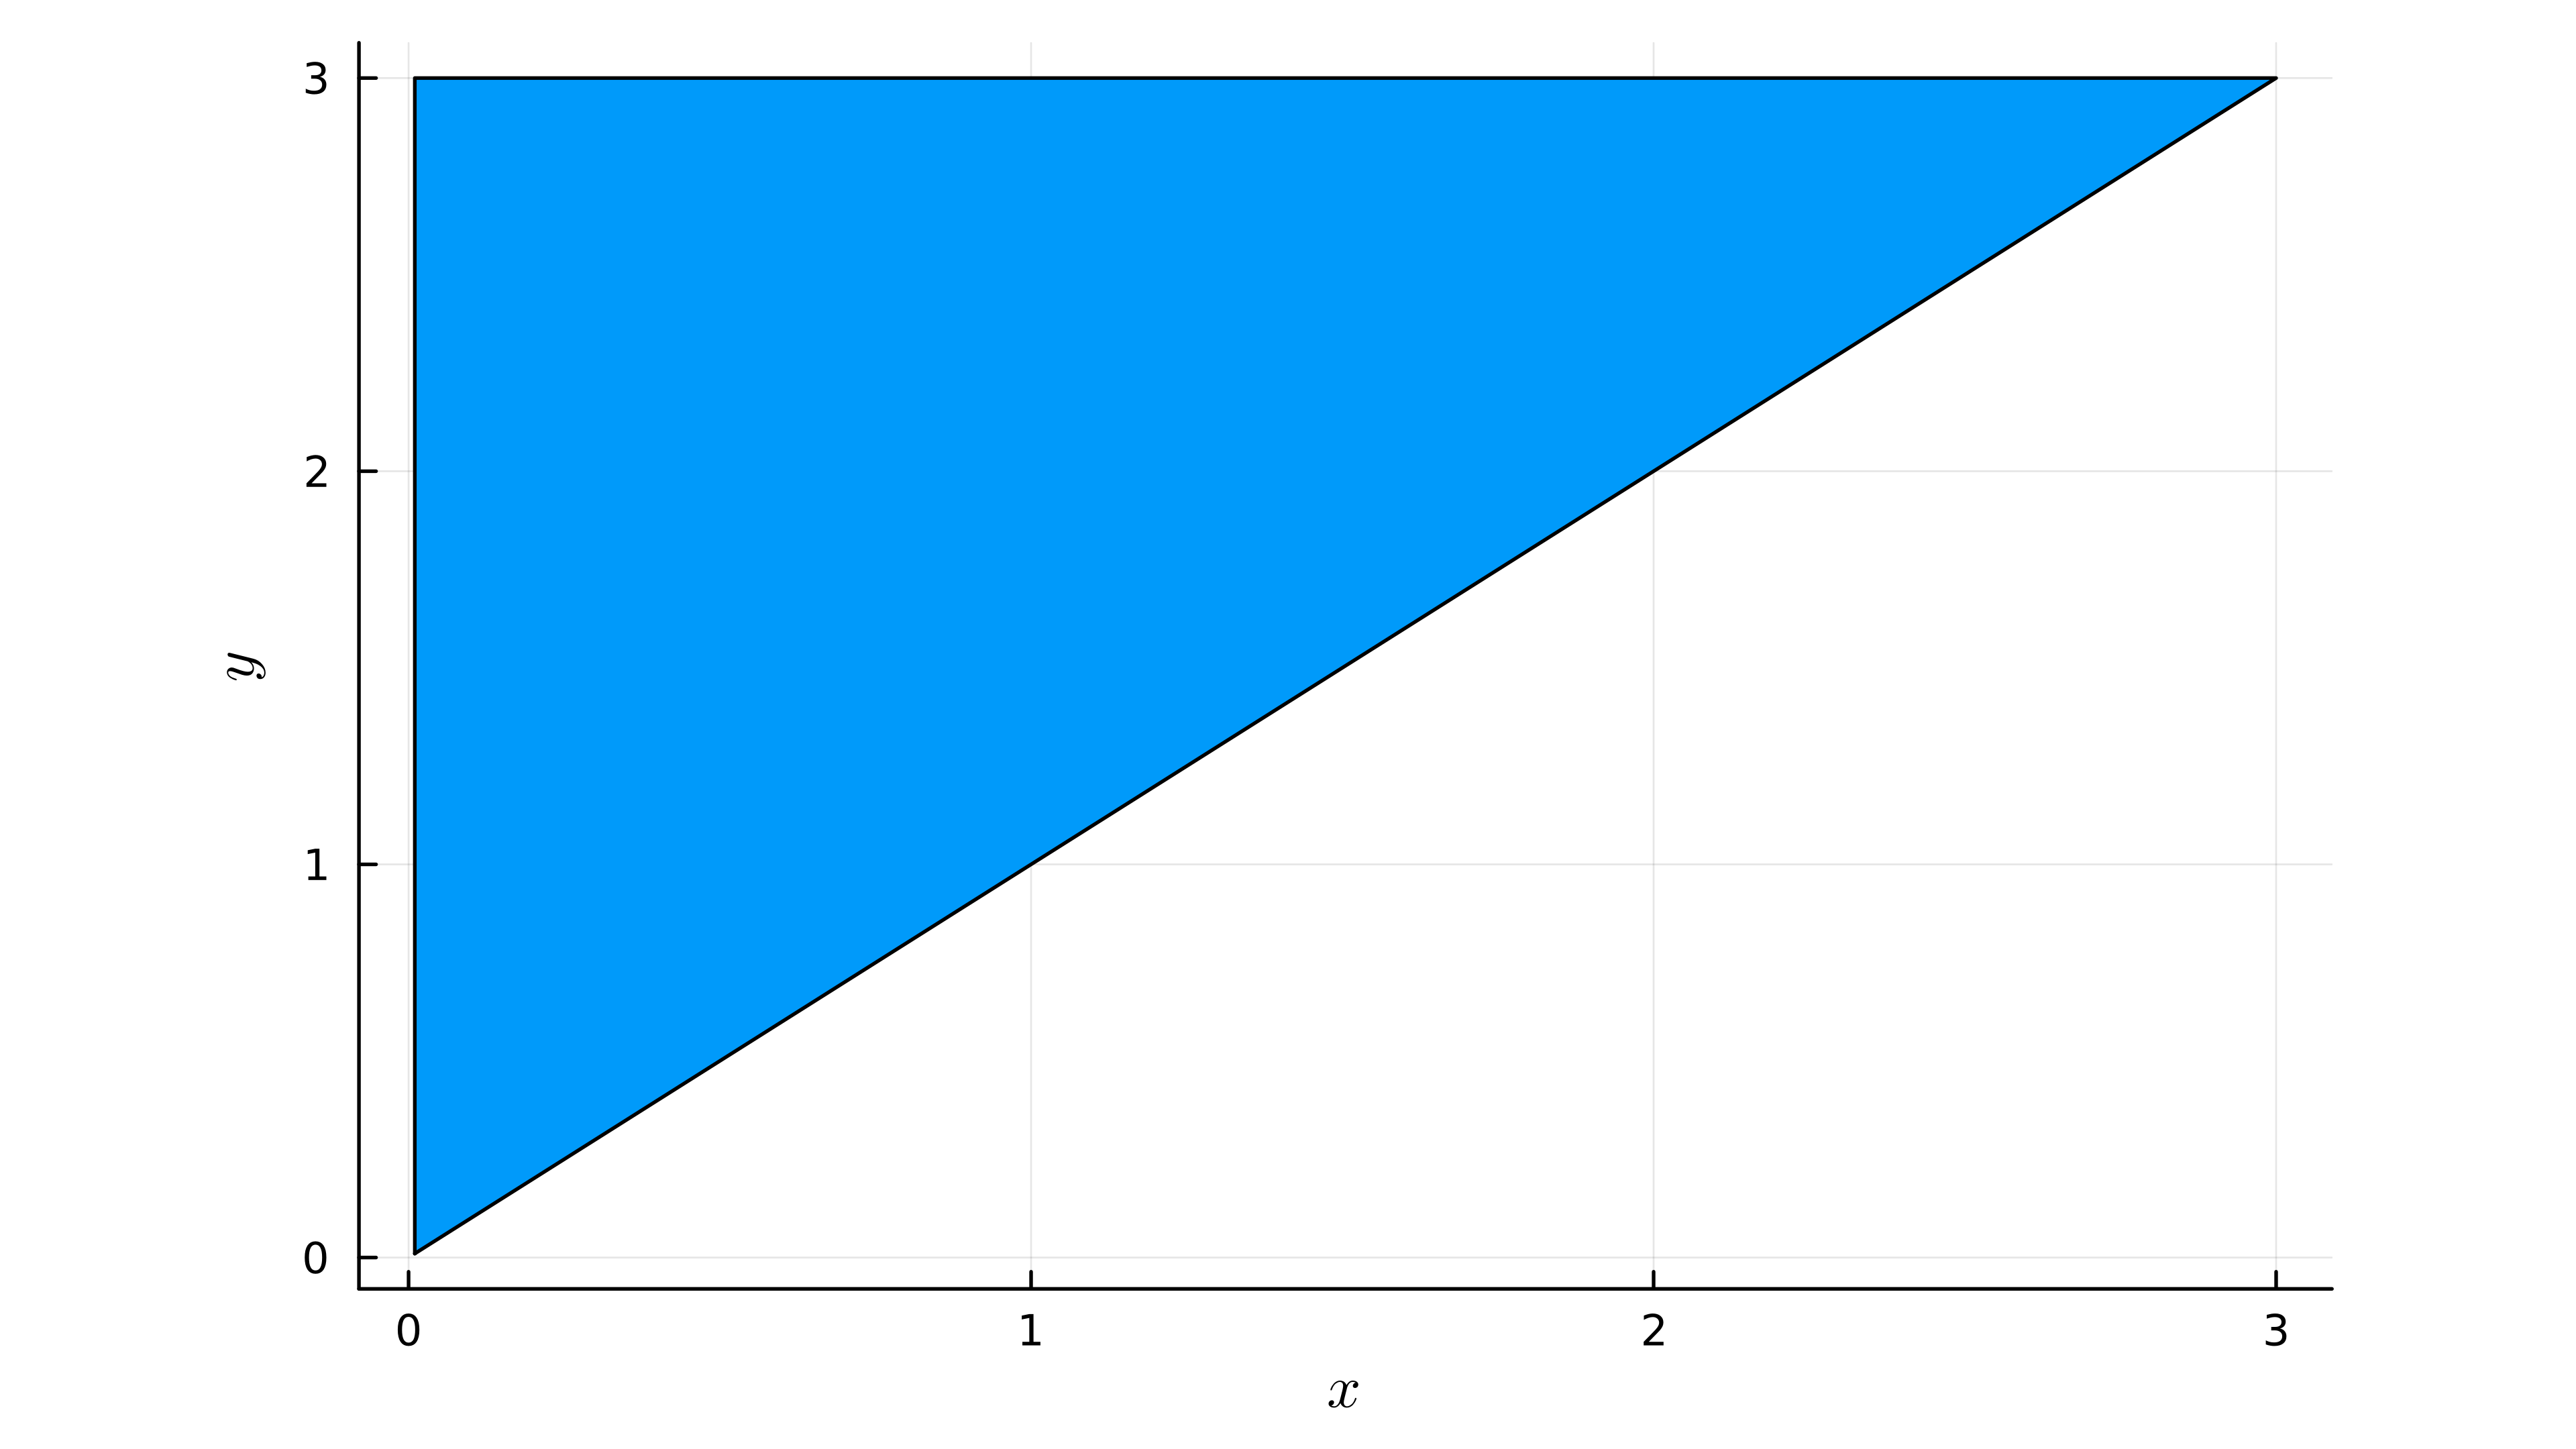
\includegraphics[scale=0.08]{figs/2.8a.png}
    \caption{Set of the item a.}
    \label{fig:2.8a}
\end{figure}

\subproblem \(\left\{ (x,y) \in \mathbb{R}_{++}^{2} \mid x/y \geq 1 \right\}\)
\subanswer

The set \(S = \left\{ \mathbf{v} \in \mathbb{R}_{++}^{2} \mid v_0/v_1 \geq 1 \right\}\), where \(\mathbf{v} = (v_0, v_1)\), is convex iff the convex combination of a pair of points belonging to \(S\), e.g., \(\mathbf{x} = (x_0, x_1)\) and \(\mathbf{y} = (y_0, y_1)\), also belong to \(S\). Mathematically,
\begin{align}
    \mathbf{w} & = \theta \mathbf{x} + (1-\theta)\mathbf{y} = \mqty[\theta x_0 + (1 - \theta)y_0 \\ \theta x_1 + (1 - \theta)y_1]
\end{align}
should belong to \(S\) to any \(\mathbf{x}, \mathbf{y} \in S\) and \(0\leq\theta\leq 1\). Therefore
\begin{align}
    \frac{\theta x_0 + (1 - \theta)y_0}{\theta x_1 + (1 - \theta)y_1} & \geq 1\\
    \theta x_0 + (1 - \theta)y_0 & \geq \theta x_1 + (1 - \theta)y_1 \\
    \frac{x_0}{x_1}\frac{\theta}{y_1} + \frac{y_0}{y_1} \frac{1 - \theta}{x_1} & \geq \frac{\theta}{y_1} + \frac{1 - \theta}{x_1}
\end{align}

This expression always holds for any value of \(\mathbf{x}, \mathbf{y} \in S\). Then, \(\mathbf{w} \in S\). The Figure \ref{fig:2.8b} shows this set for \([0, 3]\).
\begin{figure}[H]
    \centering
    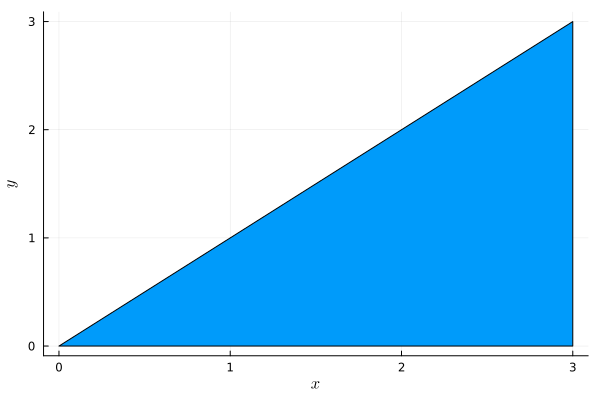
\includegraphics[scale=0.3]{figs/2.8b.png}
    \caption{Set of the item b.}
    \label{fig:2.8b}
\end{figure}

\subproblem \(\left\{ (x,y) \in \mathbb{R}_{+}^{2} \mid xy \leq 1 \right\}\)

\subanswer

If \(S = \left\{ \mathbf{v} \in \mathbb{R}_{+}^{2} \mid v_0v_1 \leq 1 \right\}\), where \(\mathbf{v} = (v_0, v_1)\), then \(S\) is convex iff
\begin{align}
    \mathbf{w} = \theta \mathbf{x} + (1-\theta)\mathbf{y} \in S \;\forall\; \mathbf{x}, \mathbf{y} \in S, 0\leq\theta\leq 1,
    \label{eq:convex-rule}
\end{align}
which is the convex combination of \(\mathbf{x}\) and \(\mathbf{y}\). Let us prove that this set is nonconvex by contradiction. Once \(\mathbf{x}, \mathbf{y} \in S\), we have that
\begin{align}
    x_0x_1 \leq 1
\end{align}
and
\begin{align}
    y_0y_1 \leq 1,
\end{align}
where \(\mathbf{x} = (x_0, x_1), \mathbf{y} = (y_0, y_1)\). The second component of \(\mathbf{w} = (w_0, w_1)\) is given by
\begin{align}
    \label{eq:2c1}
    w_1 & = \theta x_1 + (1-\theta)y_1 \\
    % w_0y_0 & = \theta x_1 y_0 + (1-\theta)y_1 y_0 \\
    % y_0 y_1 & = \frac{w_0y_0 - \theta x_1 y_0}{1-\theta} \leq 1.
\end{align}
If \(x_1 \gg 0\) and \(y_0 \gg 0\), which leads to \(x_0 \rightarrow 0\) and \(y_1 \rightarrow 0\), respectively, and \(\theta = 0.5\), then, from \eqref{eq:2c1}, we have that
\begin{align}
    w_1 & \approx 0.5 x_1.
\end{align}
Since \(x_1\) can be indiscriminality large, we have that \(w_1 \gg 0\), which leads to \(w_0 \rightarrow 0\) if \(\mathbf{w} \in S\). On the other hand, the first component of \(w_0\) is given by
\begin{align}
    \label{eq:2c2}
    w_0 & = \theta x_0 + (1-\theta)y_0 \\
    w_0 & = 0.5y_0
\end{align}

Since \(y_0\) can be indiscriminately large, we have that \(w_0 \gg 0\). However, the statement \(w_0 \rightarrow 0\) should be true in order to \(\mathbf{w}\) belong to \(S\). The contradiction leads us to conclude that \(\mathbf{w} \not\in S\). The Figure \ref{fig:2.8c} shows the set \(S\), and the Figure \ref{fig:2.8c-set} shows the cone set \(K\) in which \(\mathbf{x} \preceq_K \mathbf{w} \preceq_K \mathbf{y}\).
\begin{figure}[H]
    \centering
    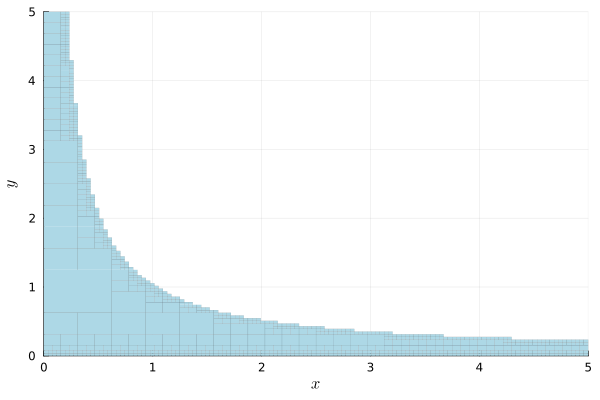
\includegraphics[scale=0.4]{figs/2.8c.png}
    \caption{Set of the item c.}
    \label{fig:2.8c}
\end{figure}

\begin{figure}[H]
    \centering
    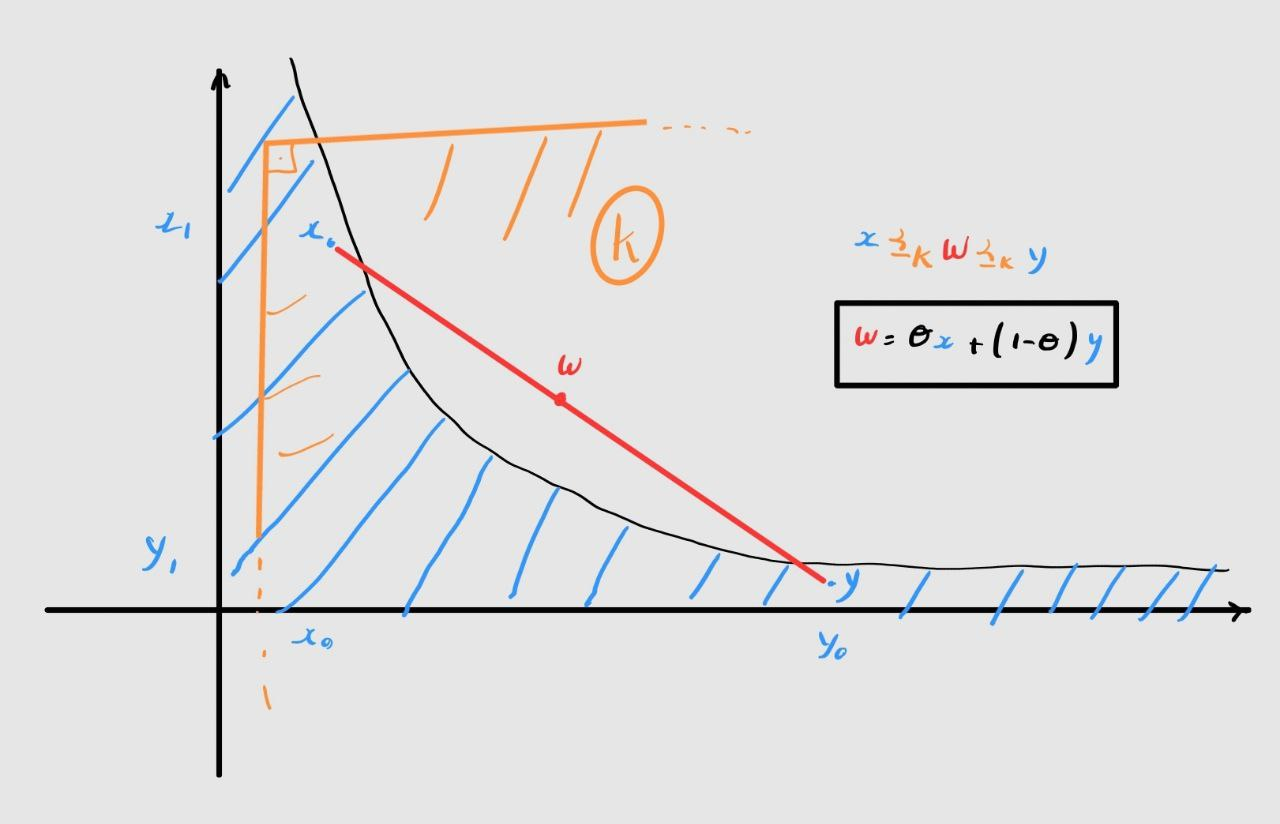
\includegraphics[scale=0.2]{figs/2.8_set.png}
    \caption{Cone set in which \(\mathbf{x} \preceq_K \mathbf{w} \preceq_K \mathbf{y}\).}
    \label{fig:2.8c-set}
\end{figure}


% Note that this set is equivalent to
% \begin{align}
%     \left\{ x \in \mathbb{R} \mid x\geq 0 \right\} \times \left\{ y \in \mathbb{R} \mid 0 \leq y \leq 1/x  \right\}.
% \end{align}

% Note that the first set is clearly linear since it is a close halfplane in \(\mathbb{R}\). If \(A = \left\{ x \in \mathbb{R} \mid x\geq 0 \right\}\), the second set is the image of \(A\) under \(f\), where
% \begin{align}
%     f(x) = \frac{1}{x}.
% \end{align}
% Mathematically,
% \begin{align}
%     B = f(A) = \left\{ y \in \mathbb{R} \mid 0 \leq y \leq 1/x  \right\}.
% \end{align}

% Once \(A\) is a convex set and \(f\) is a convex function, we conclude that \(B\) is convex. Thus, \(A \times B\) is also convex. The Figure X
% \begin{figure}[H]
%     \centering
%     \label{fig:2.8b}
%     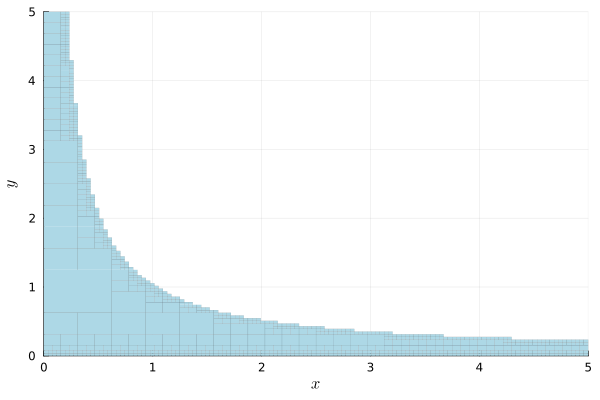
\includegraphics[scale=0.4]{figs/2.8c.png}
% \end{figure}


\subproblem  \(\left\{ (x,y) \in \mathbb{R}_{+}^{2} \mid xy \geq 1 \right\}\)

By using the convex combination, the vector \(\mathbf{w} = (w_0, w_1)\), which is given by
\begin{align}
    \mathbf{w} = \theta \mathbf{x} + (1-\theta)\mathbf{y} = \mqty[\theta x_0 + (1 - \theta)y_0 \\ \theta x_1 + (1 - \theta)y_1],
\end{align}
shall belong to \(S\), for any \(\mathbf{x}, \mathbf{y} \in S\). If it is true, then
\begin{align}
    (\theta x_0 + (1 - \theta)y_0)(\theta x_1 + (1 - \theta)y_1) & \geq 1\\
    \theta^2 x_0 x_1 + \theta(1 - \theta)y_1 x_0 + (1 - \theta)\theta x_1 y_0 + (1 - \theta)^2 y_0 y_1 & \geq 1\\
    \theta^2 x_0 x_1 + \theta(1 - \theta)(y_1 x_0 + x_1 y_0) + (1 - \theta)^2 y_0 y_1 & \geq 1 \\
    (x_0 x_1 - y_1 x_0 - x_1 y_0 + y_0 y_1 )\theta^2 + (y_1 x_0 + x_1 y_0 - 2y_0 y_1) \theta + y_0 y_1 - 1 & \geq 0 \\
    f(\theta)& \geq 0
\end{align}

Note that \(f\) is a second-order function. The previous inequation holds if \(f\) has either no roots or only one root, that is
\begin{align}
    (y_1 x_0 + x_1 y_0 - 2y_0 y_1)^2 - 4(x_0 x_1 - y_1 x_0 - x_1 y_0 + y_0 y_1 )(y_0 y_1 - 1) \geq 0 \\
    (y_1 x_0 + x_1 y_0 - 2y_0 y_1)^2 \geq 4(x_0 x_1 - y_1 x_0 - x_1 y_0 + y_0 y_1 )(y_0 y_1 - 1)
    % (y_1 x_0 + x_1 y_0 - 2y_0 y_1)^2 - 4 y_0 y_1x_0 x_1 + 4y_0 y_1^2 x_0 \nonumber \\
    % + 4y_1x_1y_0^2 - 4y_0^2 y_1^2 + 4x_0 x_1 - 4y_1 x_0 - 4x_1 y_0 + 4y_0 y_1 \geq 0 \\
    % (y_1 x_0 + x_1 y_0 - 2y_0 y_1)^2 + 4y_0 y_1^2 x_0 + 4y_1x_1y_0^2 + 4x_0 x_1 + + 4y_0 y_1 \nonumber \\
    % - 4 y_0 y_1x_0 x_1 - 4y_0^2 y_1^2 - 4y_1 x_0 - 4x_1 y_0 \geq 0 \nonumber
\end{align}
Let us analyze carefully this inequation
\begin{enumerate}
    \item If the RHS is greater than the LHS, this inequation is not satisfied. Hence, we must assess it for the worst case, where the LHS is as high as possible, and see whether this inequation holds.
    \item The worst case is when \(x_0 \gg 0\) and \(x_1 \gg 0\), and \(y_0=y_1=1\) because the term \(x_0 x_1\) cannot be quadratically compensated with \((x_0 x_1)^2\) on the LHS. Otherwise, the higher the values of \(y_0\) and \(y_1\), the lower the RHS becomes\footnote{The quadratic term \(4y_0^2 y_1^2\) on the RHS that could increase it is canceled with the very same term \(4y_0^2 y_1^2\) on the LHS.}.
    \item However, even for this case, the LHS becomes approximately equal to \((x_0 + x_1)^2 = x_0^2 + 2x_0x_1 + x_1^2\), which is greater than \(x_0x_1\)
\end{enumerate}

Therefore, the function \(f\) has no roots and the set \(\left\{ (x,y) \in \mathbb{R}_{+}^{2} \mid xy \geq 1 \right\}\) is convex. The Figure \ref{fig:2.8d} shows this set.
\begin{figure}[H]
    \centering
    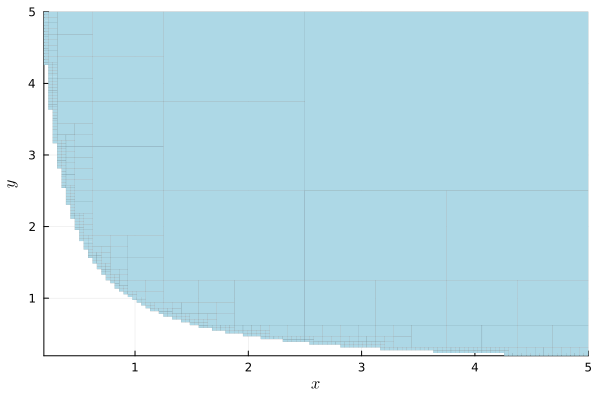
\includegraphics[scale=0.4]{figs/2.8d.png}
    \caption{Set of the item d.}
    \label{fig:2.8d}
\end{figure}

%============================================

\problem

Let \(S = \left\{\boldsymbol{\alphaup} \in \mathbb{R}^3 | \alpha_1 + \alpha_2e^{-t} + \alpha_3e^{-2t} \leq 1.1\text{ for }t \geq 1\right\}\). Is S affine, a halfspace, a convex cone, a convex set, or none of these?

The set \(S\) is affine iff its affine combination is also affine, that is,
\begin{align}
    \mathbf{w} = \theta_1 \mathbf{x} + \theta_2 \mathbf{y} = \mqty[\theta_1 x_1 + \theta_2 y_1 \\ \theta_1 x_2 + \theta_2 y_2\\ \theta_1 x_3 + \theta_2 y_3] \in S \;\forall\; \mathbf{x}, \mathbf{y} \in S, \mathbf{1}^\top\boldsymbol{\thetaup}=1,
\end{align}
where \(\boldsymbol{\thetaup} = (\theta_1, \theta_2)\), \(\mathbf{x} = (x_1, x_2, x_3)\), and \(\mathbf{y} = (y_1, y_2, y_3)\). If \(\mathbf{w} \in S\), then
\begin{align}
    \label{eq:2.15-1}
    \theta_1 x_1 + \theta_2 y_1 + (\theta_1 x_2 + \theta_2 y_2)e^{-t} + (\theta_1 x_3 + \theta_2 y_3)e^{-2t} & \leq 1.1 \nonumber \\
    \theta_1 \left( x_1 + x_2e^{-t} + x_3e^{-2t} \right) + \theta_2 \left( y_1 + y_2e^{-t} + y_3e^{-2t} \right) & \leq 1.1
\end{align}
Once \(\mathbf{x}, \mathbf{y} \in S\), \(x_1 + x_2e^{-t} + x_3e^{-2t} \leq 1.1\) and \(y_1 + y_2e^{-t} + y_3e^{-2t} \leq 1.1\), the worst case when this inequation might not be satisfied is then \(x_1 + x_2e^{-t} + x_3e^{-2t} = y_1 + y_2e^{-t} + y_3e^{-2t} = 1.1\). In this case, we have
\begin{align}
    1.1(\theta_1 + \theta_2) \leq 1.1\\
    1.1 \leq 1.1.
\end{align}

As the inequation holds, \(S\) is affine, which is consequently convex. The set \(S\) is a cone set iff the result of the conic combination also belongs to \(S\), that is,
\begin{align}
    \mathbf{w} = \theta_1 \mathbf{x} + \theta_2 \mathbf{y} = \mqty[\theta_1 x_1 + \theta_2 y_1 \\ \theta_1 x_2 + \theta_2 y_2\\ \theta_1 x_3 + \theta_2 y_3] \in S \;\forall\; \mathbf{x}, \mathbf{y} \in S, \boldsymbol{\thetaup}\succeq \mathbf{0}.
\end{align}
Recalling the Equation \eqref{eq:2.15-1}, we can clearly see that this inequation does not hold for \(\theta_1 \gg 0\), \(\theta_2 \gg 0\), and \(x_1 + x_2e^{-t} + x_3e^{-2t} = y_1 + y_2e^{-t} + y_3e^{-2t} = 1.1\). Thus, the set \(S\) is not a cone set. This set might be a close halfspace though, once halfspaces is a set of the form
\begin{align}
    \left\{ \mathbf{x} \mid \mathbf{a}^\top \mathbf{x} \leq b \right\}.
\end{align}

Considering that \(t \geq 1\) is a constant, we can rewrite \(S\) as
\begin{align}
    S = \left\{ \boldsymbol{\alphaup} \in \mathbb{R}^3 \mid \mathbf{a}^\top \boldsymbol{\alphaup} \leq b \right\},
\end{align}

where \(\mathbf{a} = (1, e^{-t}, e^{-2t})\) and \(b=1.1\). Therefore, \(S\) is a halfspace.

\problem

\subproblem Explain why \(t-(1/t)\mathbf{u}^\top \mathbf{u}\) is a concave function on \(\dom{f}\). Hint. Use convexity of the quadratic-over-linear function.

\subanswer
The function \(s_1(\mathbf{u}, t) = (1/t)\mathbf{u}^\top \mathbf{u} = \norm{\mathbf{u}}^2/t\) is a quadratic-over-linear function, which is known to be convex. The function \(s_2(\mathbf{u}, t) = t - s_1(\mathbf{u}, t)\) is a linear minus a convex function, which yields a concave function.

\subproblem From this, show that \(- \log(t - (1/t)\mathbf{u}^\top \mathbf{u})\) is a convex function on dom f.

\subanswer
Let us the define the function \(s_4(\mathbf{u}, t) = s_3 \circ s_2 = \log(s_2(\mathbf{u}, t))\), where \(s_3(x) = \log(x)\). Note that, since \(t > \norm{\mathbf{u}}\), \(\dom{s_2} = \mathbb{R}^{n}\times \mathbb{R}_{++}\) and \(s_3\) is concave and nondecreasing for this interval. As \(s_2\) is convex, we conclude by composition property that \(s_4\) is concave, thus \(s_5 = -s_4\) is convex.

\subproblem From this, show that \(f\) is convex.

\subanswer
\begin{align}
    f(\mathbf{x}, t) & = - \log(t^2 - \mathbf{x}^\top \mathbf{x}) \nonumber \\
                     & = - \log(t(t - \mathbf{x}^\top \mathbf{x}/t)) \nonumber \\
                     & = - \log(t) - \log(t - \mathbf{x}^\top \mathbf{x}/t) \nonumber \\
                     & = s_6(t) + s_5(\mathbf{u}, t).
\end{align}

We have shown that \(s_5(\mathbf{x}, t) = - \log(t - \mathbf{x}^\top \mathbf{x}/t)\) is convex. Since \(s_6(t) = - \log(t)\) is also convex on \(\dom{f}\), \(f = s_6 + s_5\) is convex as well.

\problem Square and reciprocal of convex and concave functions. For each of the following, determine if the function \(f\) is convex, concave, or neither.

\subproblem \(f(x) = g^2(x)\)

Since \(s(x) = x^2\) is convex and nondecreasing when \(g\) is nonnegative, and \(g\) is convex, then \(f = s \circ g\) is convex as well.

\subproblem \(f(x) = 1/g(x)\)

Since \(s(x) = 1/x\) is convex and nonincreasing when \(g\) is positive, and \(g\) is concave, then \(f = s \circ g\) is concave.

\problem

Let us define \(\mathbf{x}(k) \in \mathbb{R}^{n}\) and \(u(k) \in \mathbb{R}\), for \(k = 0, \dots, N-1\), as the state of a linear dynamical system and its input signal, respectively, being \(n = 3\) and \(N = 30\). The system dynamic is governed by the following equation:
\begin{align}
    \mathbf{x}(k+1) = \mathbf{A} \mathbf{x}(k) + \mathbf{b} \mathbf{u}(k),
\end{align}
where
\begin{align}
    % \mqty[\mqty{-1 & 0.4} & 0.8 \\ \mqty{\imat{2}} & \mqty{0\\0}]\\
    \mathbf{A} = \bmqty{-1 & 0.4 & 0.8\\
           1 & 0 & 0\\
           0 & 1 & 0}
\end{align}
and
\begin{align}
    \mathbf{b} = \mqty[7\\2\\-6]
\end{align}

Assuming that \(\mathbf{x}(0) = \mathbf{0}\), solve the following optimization problem:

\begin{align}
    \qq{Minimize} & \sum_{k = 0}^{N-1} f(u(k))\\
    \qq{Subject to} & \mathbf{x}(N) = \mathbf{x}_{des},
\end{align}
where
\begin{align}
    \mathbf{x}_{des} = \mqty[7\\2\\-6]
\end{align}
and
\begin{align}
    f(a) = \begin{cases}
        \abs{a} & \abs{a} \leq 1 \\
        2\abs{a} - 1 & \abs{a} > 1
    \end{cases},
\end{align}
which is equivalent to \(f(a) = \max{\left\{ \abs{a}, 2\abs{a} - 1 \right\}}\).

\answer

\begin{minted}[breaklines,escapeinside=||,mathescape=true, linenos, numbersep=3pt, gobble=2, frame=lines, fontsize=\small, framesep=2mm]{julia}
    using Convex, SCS, Plots, LaTeXStrings

    N = 30 # N in the set {0, 1, ..., N}
    n = 3 # order of the linear dynamical system
    x_des = [7, 2, -6] # constraint -> 𝐱(N) == x_des
    # model parameters
    𝐀 = [-1 .4 .8; 1 0 0; 0 1 0]
    𝐛 = [1, 0, 0.3]

    𝐗 = Variable(n, N+1) # [𝐱(0) 𝐱(1) ... 𝐱(N)]
    𝐮 = Variable(1, N) # [u(0) u(1) ... u(N-1)]
    f0 = sum(max(abs(𝐮), 2abs(𝐮)-1)) # objective function
    constraints = [
        𝐗[:,2:N+1] == 𝐀*𝐗[:,1:N]+𝐛*𝐮, # recursive equation
        𝐗[:,1] == zeros(n), # initial condition
        𝐗[:,N+1] == x_des, # final condition
    ]
    problem = minimize(f0, constraints)
    solve!(problem, SCS.Optimizer; silent_solver = true)

    fig = plot(vec(𝐮.value), xlabel=L"k", title=L"u(k)", seriestype=:sticks, markershape=:circle, label="")
    savefig(fig, "figs/4.17.png")
\end{minted}

The optimal solution of the actuator signal is shown in Figure \ref{fig:4-17}.

\begin{figure}[H]
    \centering
    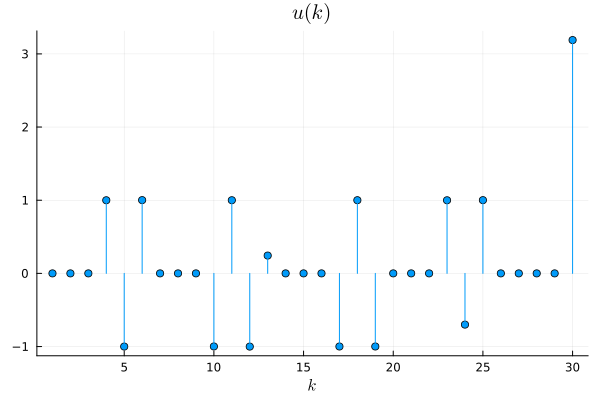
\includegraphics[scale=0.4]{figs/4.17.png}
    \caption{Optimum solution of the actuator signal.}
    \label{fig:4-17}
\end{figure}

\problem
Consider the optimization problem
\begin{align}
    \qq*{minimize} & x_1^2 \\
    \qq*{subject to} & x_1 \leq 1,\\
     & x_1^{2} + x_2^{2} \leq 2
\end{align}

with \(\mathbf{x} = (x_1, x_2)\). Determine whether each of the following statements is true or false.

\subproblem The point \((-1, 1)\) is a solution.

\subanswer True. Since \((-1, 1) \in S\), where \(S\) is the feasible set, \((-1, 1)\) is a possible solution for the problem. It is not the optimal solution, though. For this problem, \(\mathbf{x}^{\star} \approx (-1, 0)\).

\subproblem The optimal value is 1.

\subanswer True.

\begin{minted}{julia}
    using Convex, SCS

    𝐱 = Variable(2)

    f0 = square(𝐱[1]) # objective function
    constraints = [
        𝐱[1] ≤ -1,
        square(𝐱[1]) + square(𝐱[2]) ≤ 2
    ]
    problem = minimize(f0, constraints)
    solve!(problem, SCS.Optimizer; silent_solver = true)

    println(round(problem.optval, digits = 2)) # it prints 1
\end{minted}
\subproblem The problem is convex.

\subanswer True. The objective function and its domain are convex. The constraints are also convex. Then this optimization problem is convex.


\subproblem The problem has multiple solutions.
\subanswer False. Since this problem is convex, one can state that
\begin{align}
    \exists!\; \mathbf{x}^{\star} \in \mathbb{R}^{n} \mid f_0(\mathbf{x}^{\star}) \leq f_0(\mathbf{y})\;\forall\;\mathbf{y}\in S \subset \text{dom}(f),
\end{align}
where \(S\) is the feasible set.

\problem Consider the quadratic program

\begin{align}
    \qq*{minimize} & x_1^2 + x_2^2 - x_1x_2 - x_1  \nonumber \\
    \qq*{subject to}& x_1 + 2x_2 \leq u_1 \nonumber \\
     &  x_1 - 4x_2 \leq u_2 \nonumber \\
     & 5x_1 - 76x_2 \leq 1 \nonumber
\end{align}

Solve this QP, for parameter values \(u_1 = -2, u_2 = -3\), to find optimal primal variable values \(x_1^\star, x_2^\star\), and optimal dual variable values \(\lambda_1^\star, \lambda_2^\star,\) and \(\lambda_3^\star\). Let \(p^\star\) denote the optimal objective value. Verify that the KKT conditions hold for the optimal primal and dual variables you found (within reasonable numerical accuracy).

\subanswer

\begin{minted}{julia}
    using Convex, SCS
    # data parameters
    Q = [1 -1/2; -1/2 2];
    f = [-1, 0];
    A = [1 2; 1 -4; 5 76];
    b = [-2, -3, 1];
    
    
    # item 1 (a)
    x = Variable(2);
    constraints = A*x <= b;
    p = minimize(quadform(x,Q)+f'*x, constraints);
    solve!(p, SCS.Optimizer);
    lambda = constraints.dual;
    p_star = p.optval;
    println(lambda);
    println(p_star);
    println(x.value);
    println(A*x.value - b);
    println(2*Q*x.value + f + A'*lambda);
\end{minted}

\end{document}